
% Documentation of IPP
% Martin Benes
% xbenes49
% 2017/2018

\documentclass[10pt,a4paper,titlepage]{article}
\usepackage[english]{babel}
\usepackage[utf8]{inputenc}
\usepackage[margin=80pt]{geometry}


\usepackage{graphicx}   % Import pictures
\usepackage{multicol}

%\newenvironment{changemargin}[2]{%
%\begin{list}{}{%
%\setlength{\topsep}{0pt}%
%\setlength{\leftmargin}{#1}%
%\setlength{\rightmargin}{#2}%
%\setlength{\listparindent}{\parindent}%
%\setlength{\itemindent}{\parindent}%
%\setlength{\parsep}{\parskip}%
%}%
%\item[]}{\end{list}}

\begin{document}

%-----------------------------------------%
%	              DOCUMENT                  %
%-----------------------------------------%

\setcounter{page}{1}
\pagenumbering{arabic}

\begin{center}
\subsection*{Documentation of Project Implementation for IPP 2017/2018}
Name and surname: Martin Benes \\
Login: xbenes49
\end{center}

\paragraph{parse.php}
The script uses a few classes, some of them are used both in {\it parse.php}
and {\it test.php}. Firstly, there is a class hierarchy, used for input-output
operations, defined in {\it io.php}. The abstract class {\it File} implements
the common parts, its specializations {\it FileWriter} and {\it FileReader}
then have the methods, specific for them.

The class {\it Configuration} is used for procesing the arguments and
taking care of STATP extension. If the help argument occurs
in arguments, {\it HelpException} is raised.

The main part of program, compiling IPPcode18 into XML is done in {\it Compiler}.
Its {\it ProcessLine()} method is called repeatly. It returns true, when it
successfully compiled a line. When it returns false, it means program ended.
In case of error, the exception is raised. The read line is split to opcode
and arguments, and match, if for given opcode the arguments are valid
(count, types). Then using {\it Instruction} and {\it Argument} classes
it is generated to the output (the {\it FileWriter} is created by {\it Compiler}).


\paragraph{interpret.py}
In the interpret, the argument processing and reading the code is very similar
to the one in parser. There is {\it Processor} class, that process the
arguments and its method {\it NextLine()} is called for each command.

Class {\it Reader}, instantiated by {\it Processor} is a cover of XML library.
Not only it reads line by line, but it covers the jump instructions,
hence changes the read position in the code. Its method {\it decode()}
returns a callable object, representation of instruction, implemented
in {\it Instruction} class.

\begin{figure}[h!]
    \begin{center}
        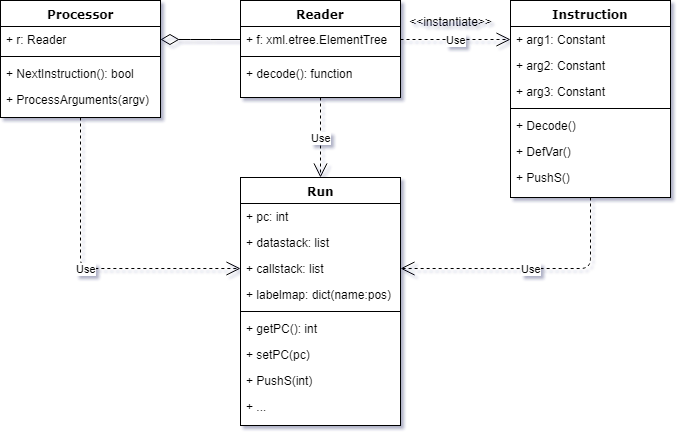
\includegraphics[width=0.4\textwidth]{interpret_classes_control.png}
        \caption{Control class diagram of interpret. \label{fig:control}}
    \end{center}
\end{figure}

Model is contained in {\it int\_model.py} module, containing three global variables
(LF, GF, TF). They are instances of {\it Frame} class, {\it LF} is an instance of
derived {\it StackFrame} class. 

Those classes contain variable objects, instances of {\it Variable} class.
The data are always represented with {\it Constant} object, even the
{\it Variable} contains Constant object in it. Inherited class 
are {\it BoolConstant}, {\it StringConstant} and {\it IntConstant},
but there is a possibility to add more types. The classes override
the methods, which are permitted for the type they represent,
otherwise the {\it SemanticException} is raised from the {\it Constant}
method implementation.


\begin{figure}[h!]
    \begin{center}
        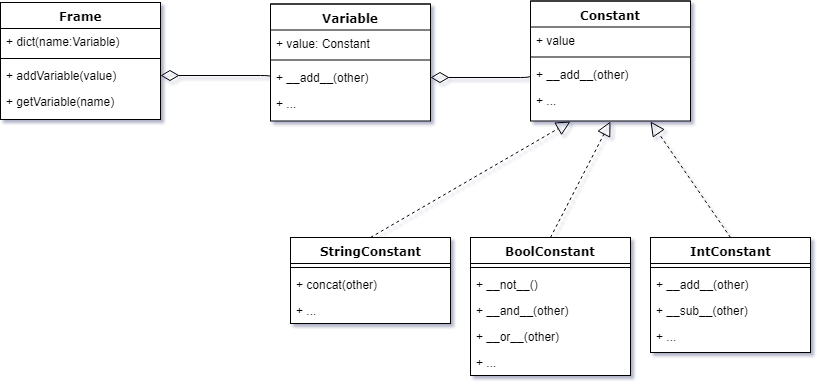
\includegraphics[width=0.5\textwidth]{interpret_classes_model.png}
        \caption{Model class diagram of interpret. \label{fig:model}}
    \end{center}
\end{figure}



\paragraph{test.php}
Firstly, it constructs {\it TestSet} and {\it TestConfig} object, that processes
the args and finds the testing files, given to the {\it TestSet} object.

Afterwards, the testing is initiated with {\it Launch()} method of
{\it TestSet} object, receiving {\it Program} object. For each test file,
its method {\it RunTest()} is called. The return value is {\it TestResult}
object, representing the result of testing.

The {\it TestResult} is then analyzed and editted, so the {\it Generator}
object, whom it is given to, could just print the HTML representation with only
a minimum of conditions. It is done at the end of program, printing the
results on standard output in HTML 5 form.

\begin{figure}[h!]
    \begin{center}
        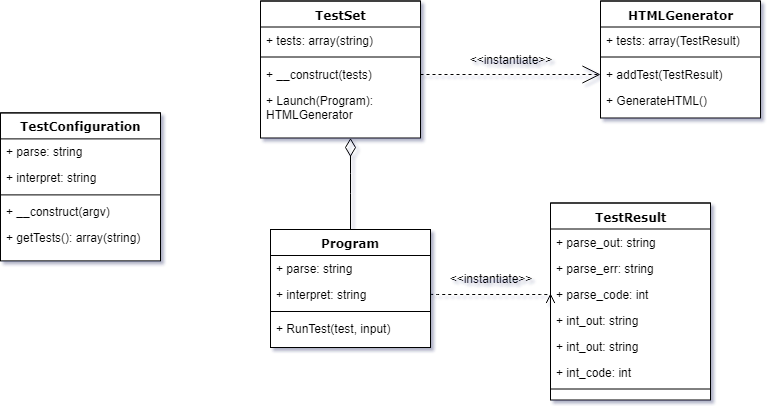
\includegraphics[width=0.6\textwidth]{test_classes.png}
        \caption{Class diagram of test. \label{fig:model}}
    \end{center}
\end{figure}

\end{document}
